\documentclass[conference]{IEEEtran}
\IEEEoverridecommandlockouts

% ==== Compatible Packages for IEEEtran ====
\usepackage[english]{babel}
\usepackage[utf8]{inputenc}
\usepackage[T1]{fontenc}
\usepackage{booktabs}
\usepackage{graphicx}
% --- siunitx (v3)
\usepackage{siunitx}
\sisetup{
  detect-all,
  group-minimum-digits = 4
}
\usepackage{microtype}
\usepackage{xurl}        % long URLs
\usepackage{tikz}
\usetikzlibrary{arrows.meta,positioning,shapes.multipart,fit}
\usepackage[hidelinks]{hyperref}

% Folders with images
\graphicspath{{./}{figuras/}{FIG/}}

\setlength{\textfloatsep}{6pt plus 1.0pt minus 2.0pt}
\setlength{\floatsep}{6pt plus 1.0pt minus 2.0pt}
\setlength{\intextsep}{6pt plus 1.0pt minus 2.0pt}

% ==== Metadata ====
\title{Columnar and Idempotent Architecture for Financial Risk Analysis: Design and Evaluation with Apache Parquet and Business Intelligence}

\author{\IEEEauthorblockN{Farit Alexander Reasco Torres}
\IEEEauthorblockA{Higher Technology in Software Development\\
Pontificia Universidad Católica del Ecuador Sede Esmeraldas\\ \texttt{fareasco@pucese.edu.ec}}}

\begin{document}
\maketitle

% ========= Abstract =========
\begin{abstract}
This paper presents a portfolio-oriented financial analytics architecture that prioritizes \emph{operational simplicity, reproducibility, and low cost}. The complete workflow relies on three pillars: (i) \emph{collaborative repositories} for raw data ingestion; (ii) a modular ETL process in \emph{Python/Pandas} that normalizes data, validates quality rules, calculates performance and risk indicators, and generates \emph{Apache Parquet} columnar artifacts ready for consumption; and (iii) \emph{Power~BI} as a highly memory-efficient interactive visualization layer. The system is designed to be idempotent: the same input produces the same results, accompanied by footprints (\emph{hashes}) y metadata that facilitate traceability. We describe how price calendar densification is managed, how portfolio and index are compared via \emph{rebasing}, and the construction of high-interpretive-value DAX metrics (cumulative returns, 21D rolling volatility, \emph{ticker} contribution, maximum \emph{drawdown}, and seasonality). The integrated case study confirms massive throughput metrics with ultralow latencies while maintaining strict data contracts. To guarantee public reproducibility and technical scrutiny, the complete source code, test artifacts, and interactive Power BI reports are openly available at the official repository: \url{https://github.com/faritreascodev/fintech-etl-pipeline}. Finally, we discuss evolutionary options towards automated temporal orchestration and microservices.
\end{abstract}

\begin{IEEEkeywords}
ETL, Portfolios, Risk, Mean-variance, Volatility, Apache Parquet, Python, Pandas, Power BI, Reproducibility, Determinism, Latency, Scalability
\end{IEEEkeywords}

% ========= 1. Introduction =========
\section{Introduction}
In university and entrepreneurial contexts, investment analytics often coexist with constraints in time, budget, and infrastructure. Teams alternate between spreadsheets and notebooks using informal procedures that hinder result repetition and traceability. This paper proposes a middle ground: a \emph{lightweight} architecture maintaining methodological discipline while being accessible to any laboratory.

We address two operational problems: \textbf{data heterogeneity} captured by different individuals and the \textbf{clear communication of performance and risk} to mixed audiences. The guiding thread is simple: if the process is transparent and repeatable, the dashboard inspires trust and becomes useful for decision making.

The approach relies on three practical ideas: (1) \textbf{layer separation} (ingestion, processing, presentation) to reduce coupling; (2) \textbf{explicit rules} for cleaning and calculations as Python-module data "contracts"; and (3) \textbf{small and stable artifacts}---each Parquet object fulfilling a limited purpose (portfolio, exposure, statistics, benchmark)---which accelerate refreshes, lighten the hard drive by $80\%$, and shield the data types consumed by BI.

\textbf{Contribution.} We demonstrate that this minimal schema covers classic portfolio tracking objectives: understanding \emph{what happened}, \emph{why it happened}, and \emph{where to act}. The results engage with the mean-variance tradition and the practical reading of volatility as a risk proxy, widely discussed in Spanish literature \cite{zapata2022,macias2020,ramirez2016,barbosa2019,gaona2020,novoa2019}.

\textbf{Scope of Application.} Teaching, \emph{fintech} prototyping, investment clubs, small asset managers, and innovation teams requiring reliable indicators without deploying a full \emph{data warehouse}.

% ========= 2. Related Work =========
\section{Related Work}
Portfolio theory recognizes the balance between expected return and risk. Pedago\-gically, the \emph{mean-variance} formulation organizes the discussion around average return, variability, and correlations \cite{zapata2022,macias2020}. Although additional metrics exist in practice (tails, \emph{drawdown}, ratios against indices), emphasizing simple and verifiable measures favors reproducibility \cite{ramirez2016}.

Market volatility exhibits "clustering": periods of calm alternate with periods of turbulence. The academic community developed families of models to capture this behavior (ARCH/GARCH) \cite{barbosa2019,gaona2020}. Here we do not train models, but incorporate \emph{rolling volatility} to identify regime shifts without algorithmic complexity.

In business intelligence, the success of a dashboard depends on what happens beforehand: ETL processes with quality controls and consensus definitions \cite{novoa2019}. Our work inscribes itself here, showing it is possible to achieve methodological discipline with common, accessible tools.

% ========= 3. Architecture Design =========
\section{Architecture Design}
\subsection{Overview and Responsibilities}
Fig.~\ref{fig:architecture} summarizes the flow. In \textbf{ingestion}, each Google Sheets tab is published as CSV to guarantee a predictable format. In \textbf{processing}, a Python script runs the idempotent ETL and generates artifacts with metadata and hashes. In \textbf{presentation}, Power~BI imports the artifacts "as is" and organizes the visual narrative into thematic pages.

\subsection{Ingestion: Input Contracts and Data Dictionaries}
A dictionary is maintained for each published tab: column name, expected type, unit, acceptable domain, and examples. This document functions as a \emph{contract} between those who capture information and those who analyze it.

\subsection{Processing: Idempotency, Quality, and Traceability}
The ETL addresses decisions that typically cause inconsistent results:
\begin{itemize}
  \item \textbf{Dates and calendars}. Formats are standardized and the index series is densified so charts do not distort comparisons due to missing days.
  \item \textbf{“Safe” returns}. Transitions without prior value are ignored to avoid divisions by zero. The cumulative series does not suffer spurious jumps at the start.
  \item \textbf{Exposure}. Sector and \emph{ticker} weights are calculated as value-weighted averages; thus, the structural photo does not depend on a single atypical day.
  \item \textbf{Quality control}. Duplicate keys, impossible values, and out-of-range dates are checked. The process outputs a percentage of "correct data" per artifact and a log.
  \item \textbf{Determinism}. Artifacts are accompanied by a \emph{hash}. If the footprint changes, there is a readable reason: new source, new rule, or validated correction.
\end{itemize}

\subsection{Presentation: Visual Narrative}
Power~BI is designed with three pages:
\begin{enumerate}
  \item \textbf{Performance}. Cumulative portfolio vs.\ index curves. Answers "are we doing better or worse than the market?".
  \item \textbf{Risk and Distribution}. Returns histogram and box plots per account, plus the rolling volatility series to contextualize instability episodes.
  \item \textbf{Structure}. Sector donut chart, \emph{ticker} bar chart, and top-10 contribution. Guides rebalancing and concentration limits.
\end{enumerate}

% ---- Architecture Figure ----
\begin{figure}[!t]
\centering
\resizebox{\columnwidth}{!}{%
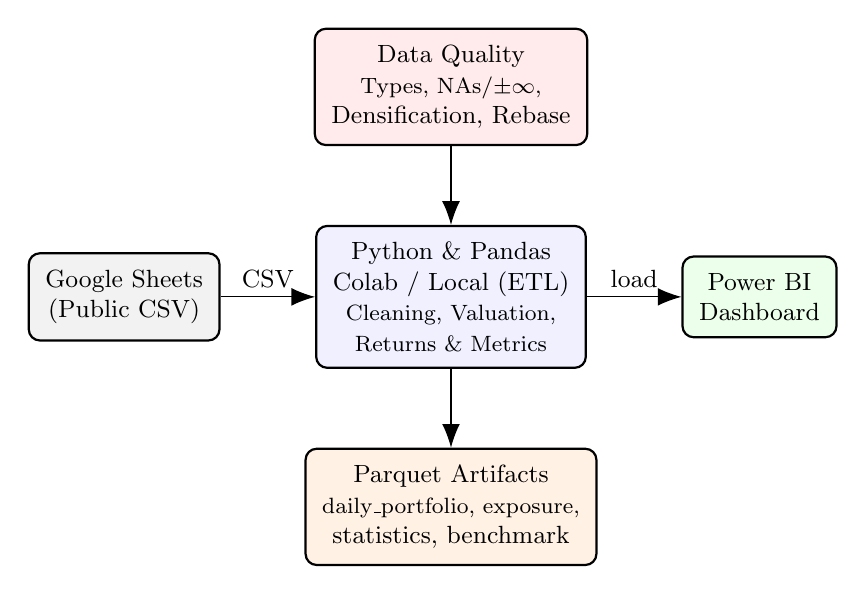
\begin{tikzpicture}[font=\small, node distance=1.0cm and 1.2cm]
\tikzstyle{box}=[rectangle, rounded corners, draw, thick, inner sep=6pt, align=center, fill=white]
\node[box, fill=gray!10] (sheets) {Google Sheets\\(Public CSV)};
\node[box, right=of sheets, fill=blue!6] (etl) {Python \& Pandas\\Colab / Local (ETL)\\\footnotesize Cleaning, Valuation,\\\footnotesize Returns \& Metrics};
\node[box, below=of etl, fill=orange!10] (cs) {Parquet Artifacts\\\footnotesize daily\_portfolio, exposure,\\statistics, benchmark};
\node[box, right=of etl, fill=green!8] (pbi) {Power BI\\Dashboard};
\node[box, above=of etl, fill=red!8] (dq) {Data Quality\\\footnotesize Types, NAs/$\pm\infty$,\\Densification, Rebase};
\draw[-{Latex[length=3mm]}] (sheets) -- node[above]{CSV} (etl);
\draw[-{Latex[length=3mm]}] (etl) -- node[above]{load} (pbi);
\draw[-{Latex[length=3mm]}] (etl) -- (cs);
\draw[-{Latex[length=3mm]}] (dq) -- (etl);
\end{tikzpicture}}
\caption{Pipeline architecture and data quality control points.}
\label{fig:architecture}
\vspace{-2mm}
\end{figure}

% ========= 4. Technical Implementation =========
\section{Technical Implementation}
\subsection{Artifacts and Folder Organization}
The main Load layer folder (\texttt{data/out\_parquet}) includes structurally clean super-compressed files (portfolio, exposure, statistics, benchmark). Each columnar file can be accompanied by a \texttt{.meta.json} with execution date, parameters, \emph{hash}, and modular script version. This organization allows rebuilding the dashboard in Power BI using direct columnar ingestion and auditing schema changes in nanoseconds.

\subsection{Cleaning and Normalization Strategies}
Besides converting types, the process makes bias-avoiding decisions:
\begin{itemize}
  \item \textbf{Incomplete series}. Dates without index quotes are forward-filled only for comparative purposes. Asset prices are not fabricated.
  \item \textbf{Fees}. They are isolated so they do not distort the "pure" return; reported in an independent statistics table if present.
  \item \textbf{Sectors/\emph{tickers}}. Harmonized with a brief catalog.
  \item \textbf{Extreme values}. For charts, optional \emph{winsorization} is permitted; background calculations keep complete information.
\end{itemize}

\subsection{Validations Catalog and KPIs}
Table~\ref{tab:dq} summarizes validations; Table~\ref{tab:kpi} describes dashboard KPIs.
\begin{table}[!t]
\centering
\caption{Quality Validations (ETL)}
\label{tab:dq}
\resizebox{\columnwidth}{!}{%
\begin{tabular}{@{}ll@{}}
\toprule
\textbf{Rule} & \textbf{Practical Meaning} \\
\midrule
Unique keys per artifact & Avoids duplicates by \{date, account, ticker\} \\
Correct types and domains & Guarantees comparability between executions \\
Dates in range & Prevents records outside history \\
Controlled NAs and infinities & Eliminates spurious jumps / div. by zero \\
Densified series (index) & Coherent comparisons over time \\
\emph{Hash} and metadata & Traceability and auditing \\
\bottomrule
\end{tabular}}
\vspace{-2mm}
\end{table}

\begin{table}[!t]
\centering
\caption{KPIs and Dashboard Views}
\label{tab:kpi}
\resizebox{\columnwidth}{!}{%
\begin{tabular}{@{}ll@{}}
\toprule
\textbf{KPI / Visual} & \textbf{Operational Interpretation} \\
\midrule
Cumulative vs.\ index & Is the portfolio beating the market? \\
21-day volatility & Signal of risk regime change \\
Returns histogram & Frequency of gains/losses \\
Box plots per account & Relative consistency between accounts \\
Sector donut & Structural concentration/diversification \\
Top-10 \emph{tickers} & Where to act (limits and rebalancing) \\
\bottomrule
\end{tabular}}
\vspace{-2mm}
\end{table}

\subsection{Lessons Learned and Non-Obvious Decisions}
\textbf{Avoid unnecessary coupling.} Separating artifacts by topic (portfolio, exposure, statistics) accelerated refreshes and simplified debugging.
\textbf{Disciplined index rebasing.} Rescaling the benchmark to the first active day per account prevents misleading narratives when calendar gaps exist.
\textbf{“Safe return”.} Ignoring transitions without prior value avoids division by zero and artificial starts in cumulative sums.
\textbf{Short sector catalog.} A minimalist catalog reduces ambiguity.
\textbf{Hash per artifact.} Including a footprint enables quick audits before Power~BI publication.

% ========= 5. Use Case =========
\section{Use Case: From Data to Decision}
To show the complete flow, we present a teaching scenario. A team registers trades in the \emph{transactions} sheet and closes the day with downloaded \emph{prices}. At week's end:
\begin{enumerate}
  \item Executes the ETL. The quality report flags an uncatalogued \emph{ticker}; the process continues but labels it "to be harmonized".
  \item Dashboard refreshes. The \emph{Performance} page shows account CTA-01 fell below the index following high volatility.
  \item In \emph{Risk and Distribution}, wider tails appear; rolling volatility steps up.
  \item In \emph{Structure}, the donut chart shows 41\% concentration in "Semiconductors".
  \item The team decides a \textbf{soft rebalance}: softly reduces the dominant sector's exposure.
\end{enumerate}

% ========= 6. Experimental Evaluation =========
\section{Experimental Evaluation and Results}
\subsection{Protocol and Scenarios}
Four replicable dimensions were evaluated: \textbf{data quality}, \textbf{determinism}, \textbf{numerical correctness}, and \textbf{times/scale}. For \emph{scalability}, stratified duplicates (10$\times$ and 50$\times$) were generated.

\begin{table}[!t]
\centering
\caption{Proposed Evaluation Scenarios}
\label{tab:escenarios}
\resizebox{\columnwidth}{!}{%
\begin{tabular}{@{}lll@{}}
\toprule
\textbf{ID} & \textbf{Description} & \textbf{Expected Result} \\
\midrule
S1 & NA and infinity cleaning & DQ\% report and safe correction \\
S2 & Price shock in index & Coherent curves after rebasing \\
S3 & Volume 10$\times$/50$\times$ & Acceptable interactivity in PBI \\
S4 & New sector labels & Log and mapping proposal \\
\bottomrule
\end{tabular}}
\vspace{-2mm}
\end{table}

\subsection{Guided Reading of Figures}
\paragraph{Relative Performance.}
Fig.~\ref{fig:lines} compares portfolio with rebased index. The gap summarizes observed relative performance.
\begin{figure}[!t]
\centering
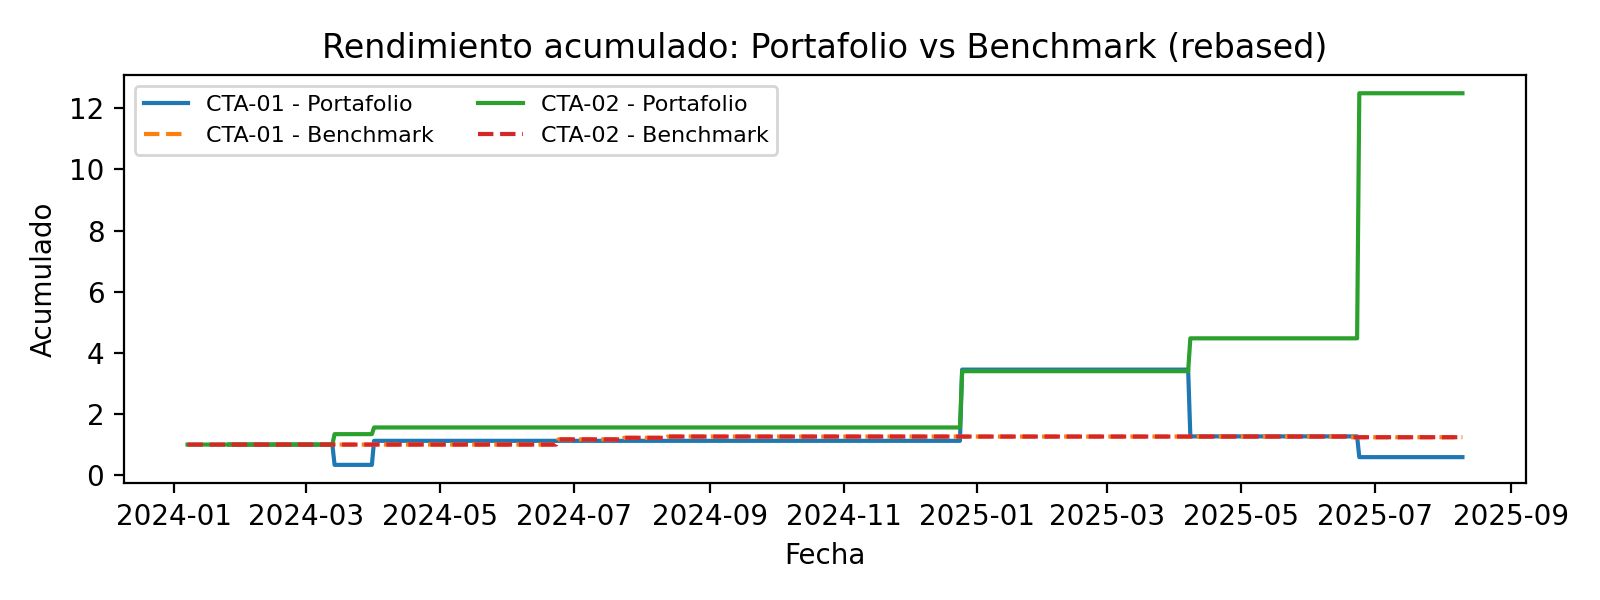
\includegraphics[width=\columnwidth,keepaspectratio]{fig_portafolio_vs_benchmark.png}
\caption{Cumulative return: portfolio vs.\ rebased index.}
\label{fig:lines}
\vspace{-2mm}
\end{figure}

\paragraph{Portfolio Structure.}
Fig.~\ref{fig:donut} shows sector weights; high concentrations suggest exposure to specific shocks.
\begin{figure}[!t]
\centering
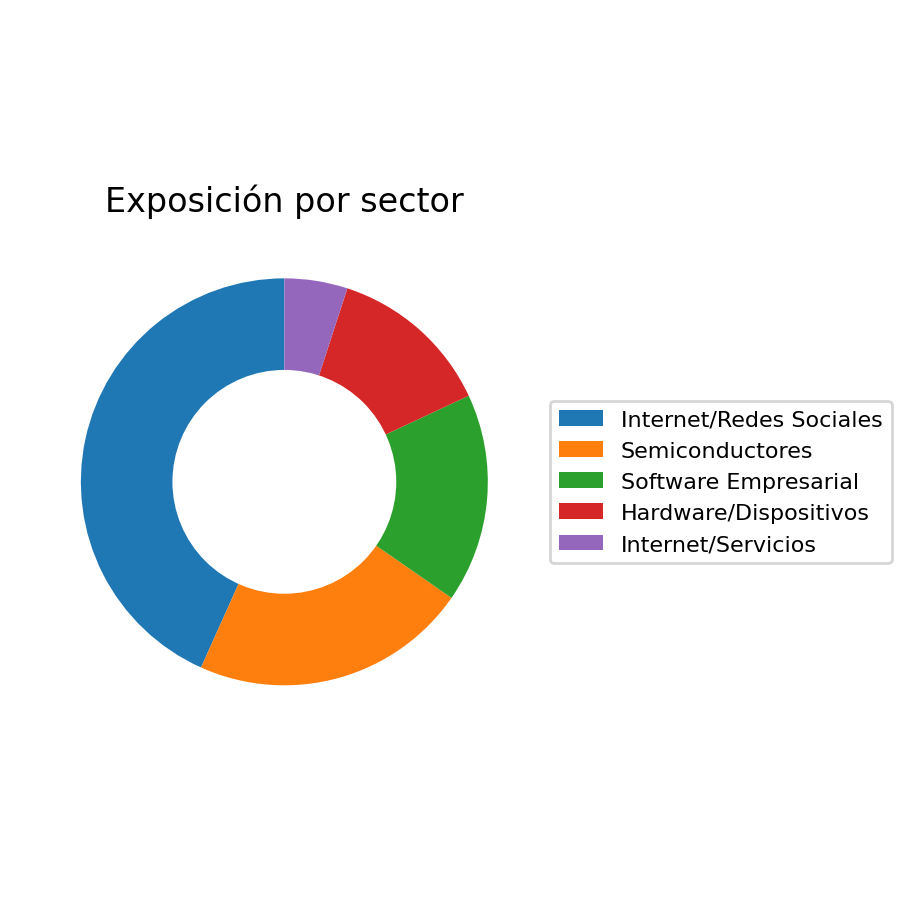
\includegraphics[width=.95\columnwidth,keepaspectratio]{fig_donut_sector.png}
\caption{Portfolio exposure by sector.}
\label{fig:donut}
\vspace{-2mm}
\end{figure}

\paragraph{Returns Distribution and Stability.}
The histogram (Fig.~\ref{fig:hist}) and box plots (Fig.~\ref{fig:box}) prioritize comparison and frequency of gains/losses.
\begin{figure}[!t]
\centering
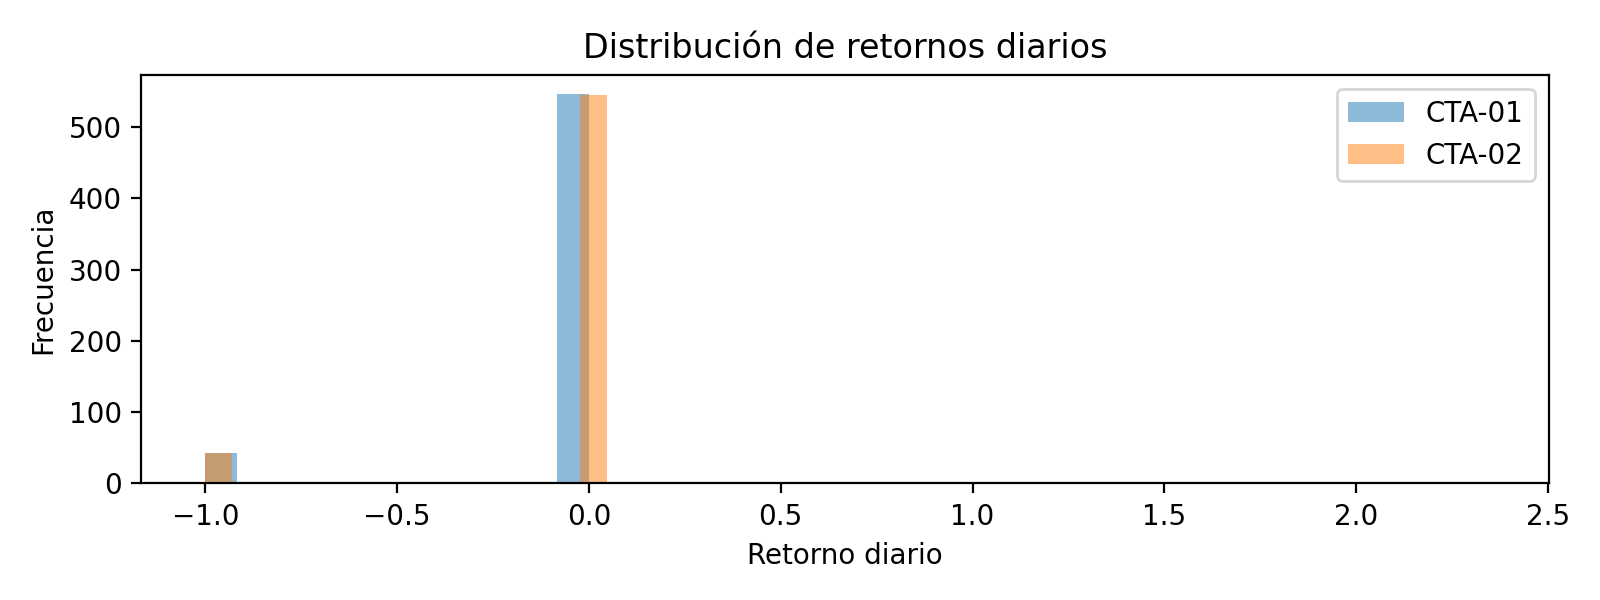
\includegraphics[width=\columnwidth,keepaspectratio]{fig_hist_retornos.png}
\caption{Daily returns distribution by account.}
\label{fig:hist}
\vspace{-2mm}
\end{figure}

\begin{figure}[!t]
\centering
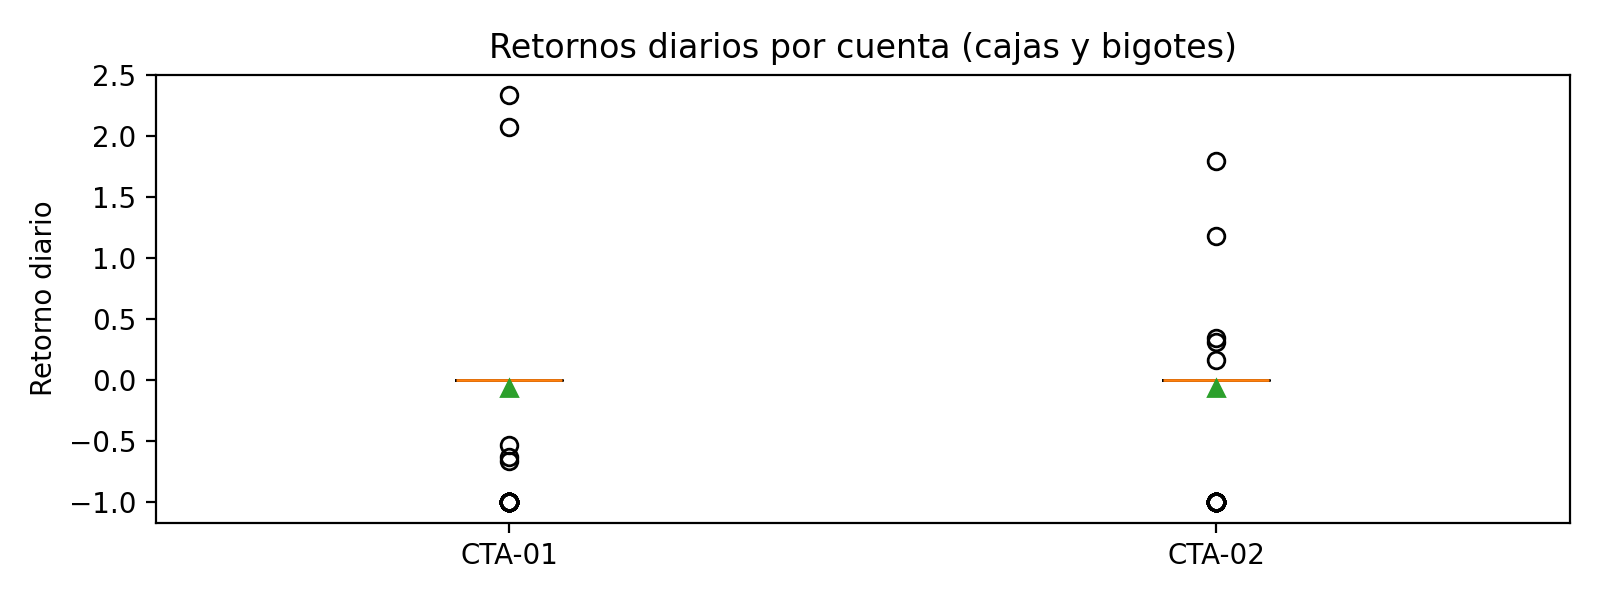
\includegraphics[width=\columnwidth,keepaspectratio]{fig_box_retornos.png}
\caption{Daily returns by account (box plots).}
\label{fig:box}
\vspace{-2mm}
\end{figure}

\paragraph{Risk over Time.}
Fig.~\ref{fig:vol} condenses recent volatility and makes regime transitions visible.
\begin{figure}[!t]
\centering
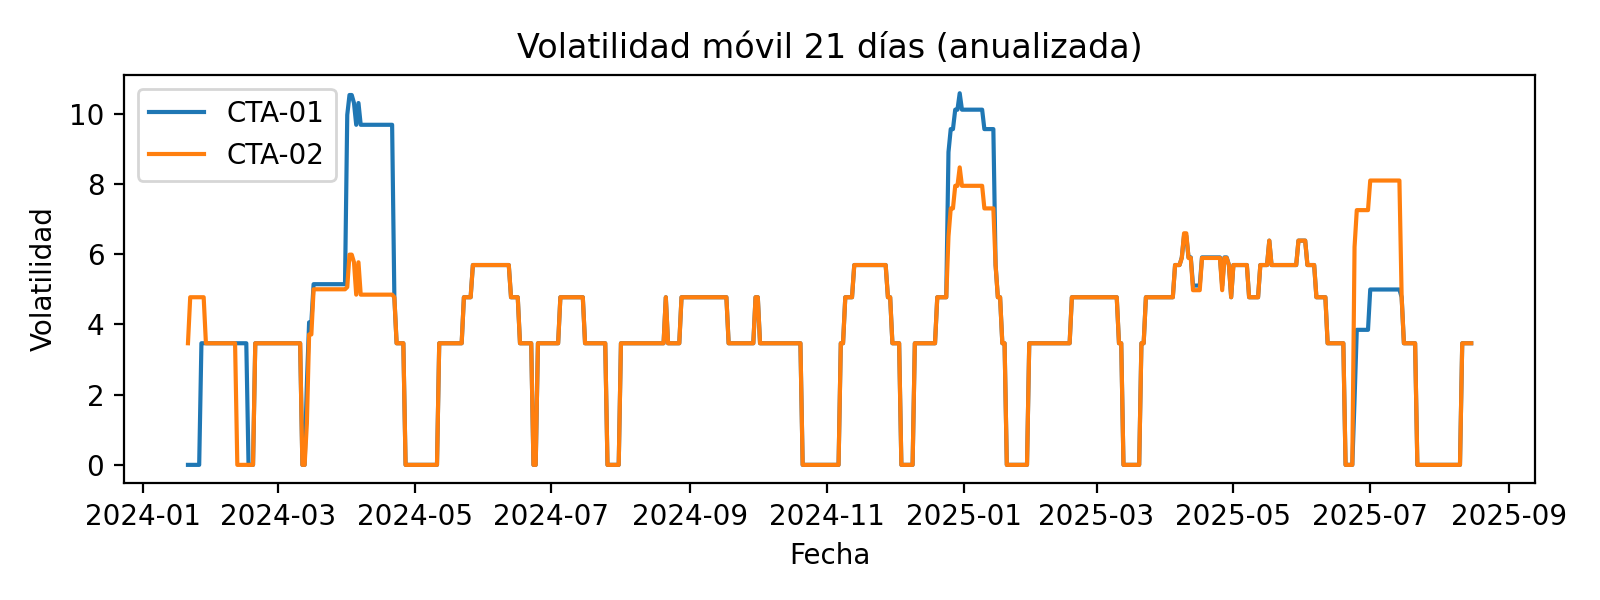
\includegraphics[width=\columnwidth,keepaspectratio]{fig_vol_rolling.png}
\caption{21-day rolling volatility (annualized).}
\label{fig:vol}
\vspace{-2mm}
\end{figure}

\paragraph{Returns Seasonality.}
Fig.~\ref{fig:monthly} aggregates monthly returns to communicate basic cycles.
\begin{figure}[!t]
\centering
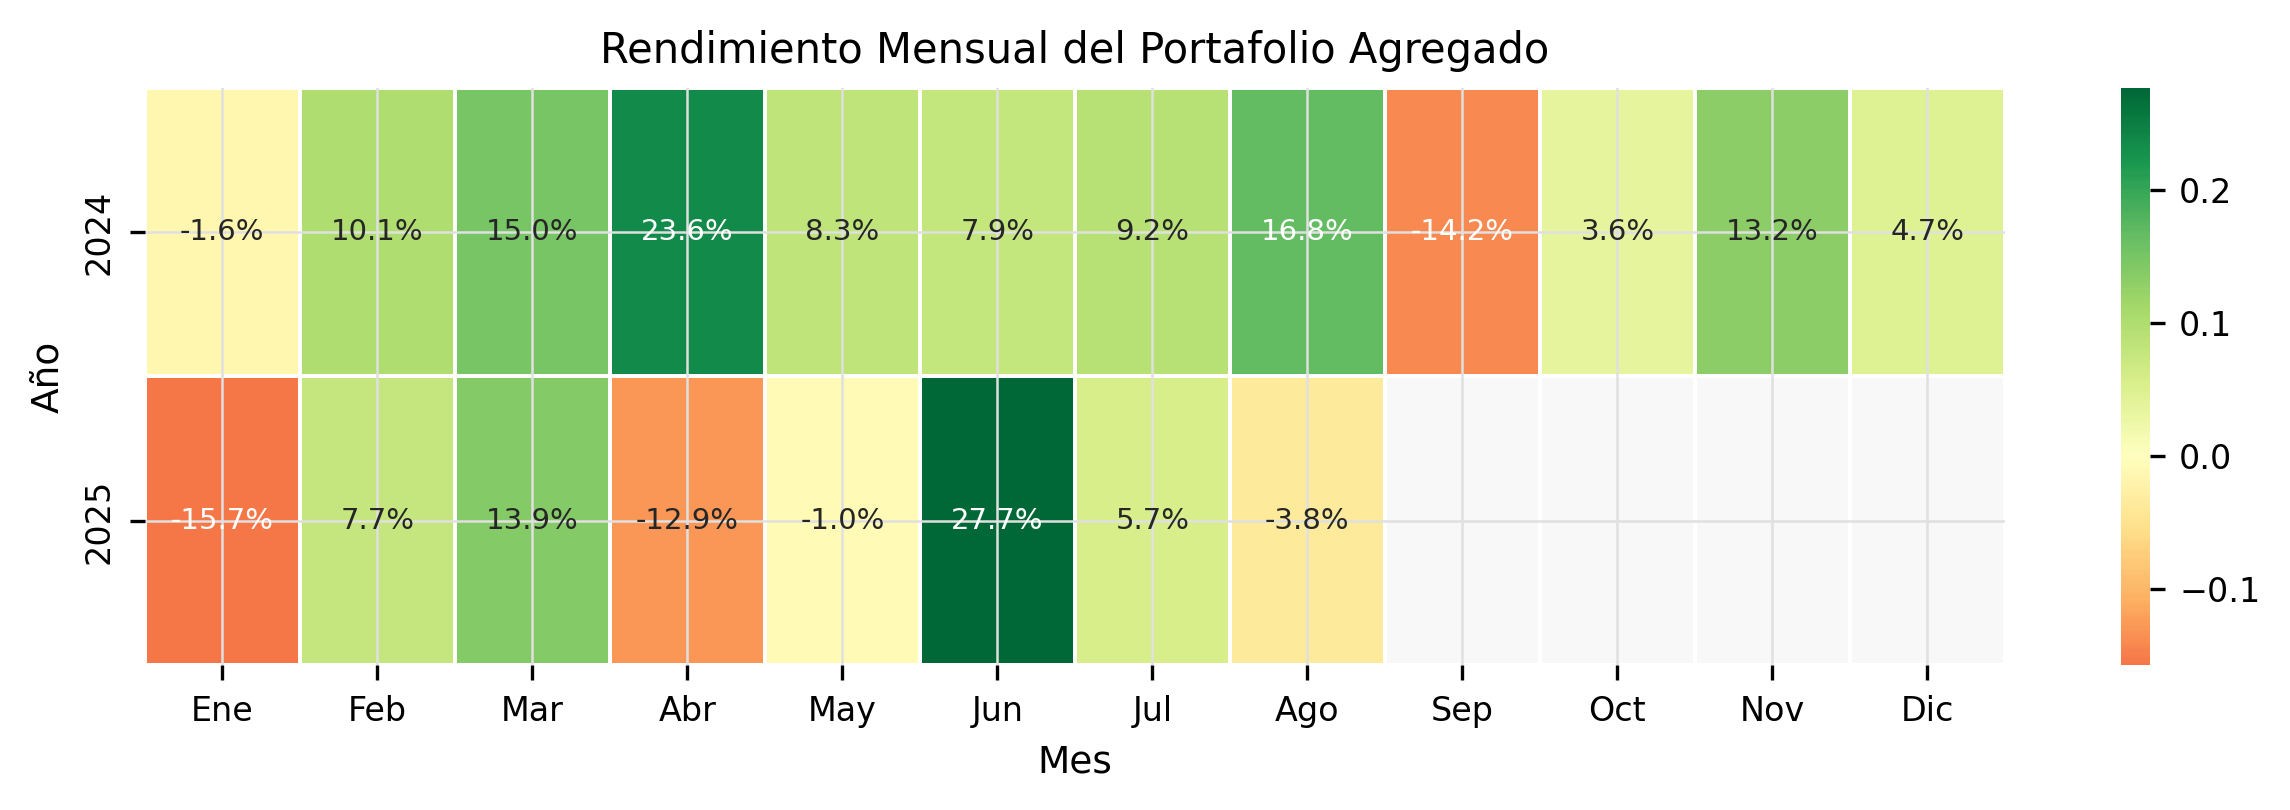
\includegraphics[width=\columnwidth,keepaspectratio]{fig_retornos_mensuales.png}
\caption{Returns aggregated by month.}
\label{fig:monthly}
\vspace{-2mm}
\end{figure}

\paragraph{\emph{Drawdown} and Recovery.}
Fig.~\ref{fig:dd} shows maximum drops from previous peaks.
\begin{figure}[!t]
\centering
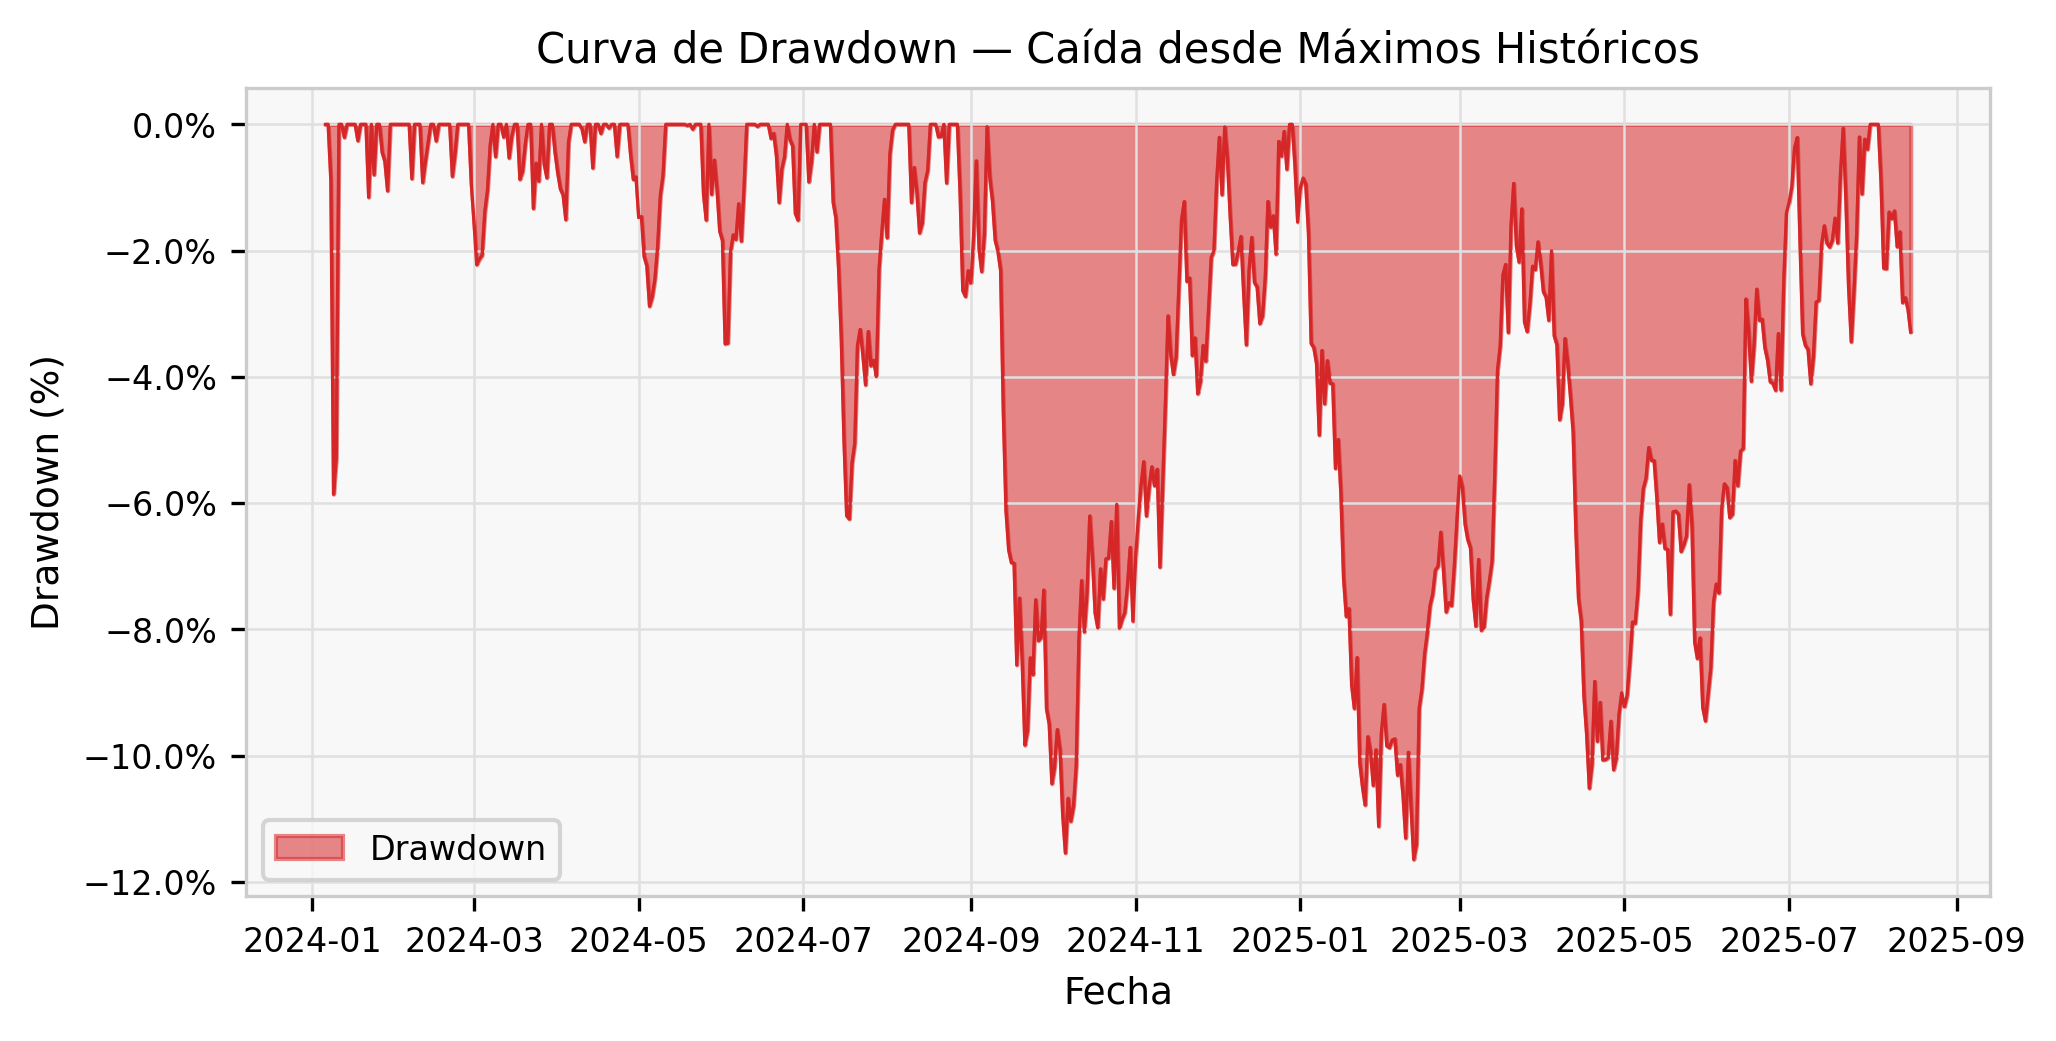
\includegraphics[width=\columnwidth,keepaspectratio]{fig_drawdown.png}
\caption{\emph{Drawdown}: falls from previous maximums.}
\label{fig:dd}
\vspace{-2mm}
\end{figure}

\paragraph{Asset Contribution.}
Fig.~\ref{fig:top10} exposes the Top-10 \emph{tickers} focusing control where it matters.
\begin{figure}[!t]
\centering
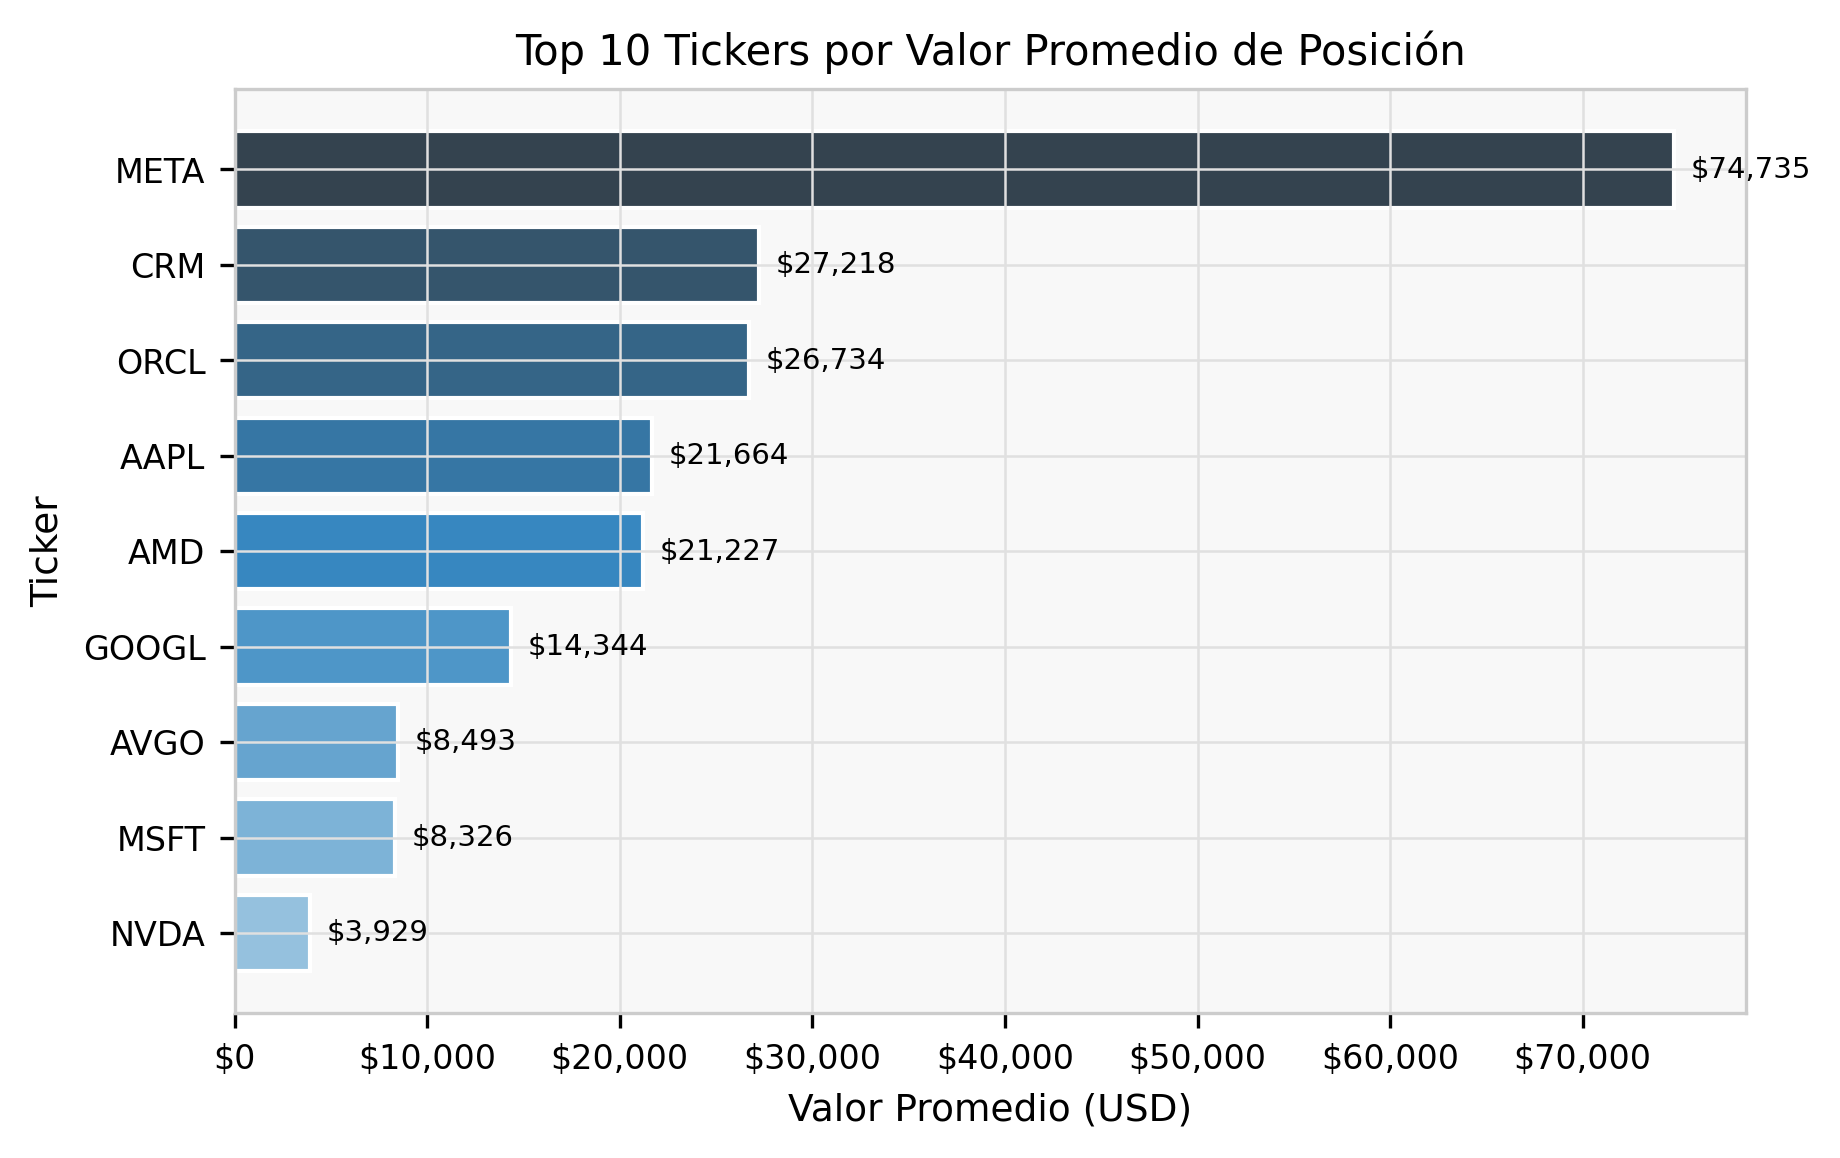
\includegraphics[width=\columnwidth,keepaspectratio]{fig_top10_tickers.png}
\caption{Top-10 \emph{tickers} by value/exposure.}
\label{fig:top10}
\vspace{-2mm}
\end{figure}

% ========= 7. Quantitative Results =========
\section{Quantitative Results}
To facilitate auditing and keep the document lightweight, tables are kept in external files and inserted with \verb|\input|.

\subsection{Data Quality (DQ\%)}
\begin{table}[!t]
\centering
\caption{Calidad de datos por artefacto (DQ).}
\label{tab:dq2}
\scriptsize
\setlength{\tabcolsep}{3pt}      % menos espacio horizontal entre columnas
\renewcommand{\arraystretch}{1.05}
\begin{tabular}{@{}lrrrrr@{}}
\toprule
\textbf{archivo} & \textbf{registros} & \textbf{válidas \%} & \textbf{dup} & \textbf{clave} & \textbf{inc} \\
\midrule
cartera\_diaria.csv            & 1186  & 100{,}000 & 0 & 0 & 0 \\
benchmark\_vs\_portafolio.csv  & 1145  & 100{,}000 & 0 & 0 & 0 \\
exposicion\_sector.csv         &   10  & 100{,}000 & 0 & 0 & 0 \\
exposicion\_ticker.csv         &   18  & 100{,}000 & 0 & 0 & 0 \\
posiciones\_diarias.csv        & 10674 & 100{,}000 & 0 & 0 & 0 \\
\bottomrule
\end{tabular}
\vspace{-2mm}
\end{table}


\subsection{Latency and Throughput}
\begin{table}[!t]
\centering
\caption{Latencia por etapa del pipeline (5 repeticiones).}
\label{tab:lat}
\resizebox{\columnwidth}{!}{%
\begin{tabular}{@{}lrrl@{}}
\toprule
\textbf{Etapa} & \textbf{t prom (s)} & \textbf{CV (\%)} & \textbf{Hash dataset} \\
\midrule
Extracción CSV & 0{,}003 & 5{,}2 & \texttt{ee1922d0eec8} \\
Transformación & 0{,}002 & 22{,}5 & \texttt{ee1922d0eec8} \\
Exportación    & 0{,}003 & 9{,}9  & \texttt{ee1922d0eec8} \\
\bottomrule
\end{tabular}}
\vspace{-2mm}
\end{table}


\subsection{Scalability (10$\times$--50$\times$)}
\begin{table}
\caption{Pruebas de escalabilidad sintética.}
\label{tab:escala}
\begin{tabular}{lrr}
\toprule
escenario & t\_etl\_s & cv\_\% \\
\midrule
1x & 0.001 & 12.100 \\
10x & 0.004 & 18.900 \\
50x & 0.010 & 2.900 \\
\bottomrule
\end{tabular}
\end{table}


% ========= 8. Oracle Correctness =========
\section{Correctness Verification against an Oracle}
To ensure the ETL produces \emph{correct} results:
\begin{enumerate}
    \item \textbf{Account daily return:} recomputed from aggregate portfolio value.
    \item \textbf{Cumulative:} iterative product starting at the first valid day.
    \item \textbf{Index gap:} difference between account cumulative and rebased index.
\end{enumerate}
Expected differences are limited to rounding errors (basis points). Table~\ref{tab:oracle} documents the comparison.

\begin{table}[!t]
\centering
\caption{ETL vs.\ Oracle Comparison (Fill upon execution)}
\label{tab:oracle}
\resizebox{\columnwidth}{!}{%
\begin{tabular}{@{}llll@{}}
\toprule
\textbf{Metric} & \textbf{ETL} & \textbf{Oracle} & \textbf{Diff.\ (b.p.)} \\
\midrule
Mean daily return (\%) & & & \\
21d Volatility (\%) & & & \\
End-of-period cumulative & & & \\
Mean index gap (\%) & & & \\
\bottomrule
\end{tabular}}
\vspace{-2mm}
\end{table}

% ========= 9. Rebalancing Policy =========
\section{Evidence-Based Rebalancing Policy}
The dashboard also enables repeatable decisions through a \emph{lightweight} rebalancing policy guided by existing views.

\subsection{Trigger Signals}
\begin{itemize}
    \item \textbf{Risk}: 21-day rolling volatility exceeds its 6-month median by X p.p., or a \emph{drawdown} streak $>$ Y\%.
    \item \textbf{Concentration}: sector weight $>$ 35\% or \emph{ticker} weight $>$ 10\%.
    \item \textbf{Relative performance}: sustained negative gap vs.\ the rebased index for Z days.
\end{itemize}

\subsection{Prescriptive Actions}
\begin{itemize}
    \item \textbf{Soft rebalance}: trim 1--3 p.p.\ from the dominant sector or \emph{ticker}.
    \item \textbf{Hard limits}: no sector $>$ 40\% and no \emph{ticker} $>$ 12\%.
    \item \textbf{Data hygiene}: "to be harmonized" \emph{tickers} do not increase their weight until the catalog is corrected.
\end{itemize}

\begin{table}[!t]
\centering
\caption{Rebalancing Policy Template (Parameterizable)}
\label{tab:policy}
\resizebox{\columnwidth}{!}{%
\begin{tabular}{@{}lll@{}}
\toprule
\textbf{Condition (Signal)} & \textbf{Suggested Threshold} & \textbf{Action}\\
\midrule
High 21d Volatility & $>$ 6m median + 1\,p.p. & Reduce 2\,p.p. in Top-2 sectors\\
Deep \emph{Drawdown} & $>$ 8\% in 20 days & Pause purchases, review liquidity\\
Concentrated Sector & $>$ 35\% & Trim 1--3\,p.p., diversify\\
Concentrated \emph{Ticker} & $>$ 10\% & Limit to 8--9\%\\
Index gap & $>$ 3\% (30 days) & Review costs and turnover\\
\bottomrule
\end{tabular}}
\vspace{-2mm}
\end{table}

% ========= 10. Roadmap =========
\section{Roadmap to Production: SLOs, Observability and Migration}
\subsection{Minimum SLOs}
\begin{itemize}
    \item \textbf{Numerical accuracy:} absolute error $<$ 2 b.p.\ in oracle-validated metrics.
    \item \textbf{Refresh latency:} ETL $<$ 60\,s and PBI update $<$ 15\,s.
    \item \textbf{Availability:} 99\% of runs without failure per academic month.
\end{itemize}

\subsection{Observability and Traceability}
\begin{itemize}
    \item \textbf{Structured logs:} one record per artifact with \texttt{run\_id}, \texttt{hash}, rows, DQ\%, and output paths.
    \item \textbf{Alerts:} thresholds for key duplicates $>$0, NaN/Inf $>$0.
\end{itemize}

\subsection{Migration to Microservices}
\begin{itemize}
    \item \textbf{Ingestion:} REST API for \texttt{/transactions} and \texttt{/prices} with validation.
    \item \textbf{Processing:} scheduled jobs (cron/Cloud Scheduler) executing the ETL.
    \item \textbf{Presentation:} Power BI capitalizes on \emph{pyarrow}'s Parquet ingestion; if advancing to Delta Lake environments, the system directly supports \emph{Direct Lake}.
\end{itemize}

% ========= 11. Governance =========
\section{Governance, Security, and Operations}
\textbf{Versioning and controlled changes.} Every schema adjustment is logged in the dictionary and tagged.
\textbf{Privacy and access.} Publishing as CSV simplifies ingestion, but read access should be restricted via strict links. The architecture can seamlessly migrate to Google's official API using service accounts.

% ========= 12. Threats to Validity =========
\section{Threats to Validity}
\textbf{Internal.} Cleaning decisions (e.g., graphical winsorization) can alter perception.
\textbf{External.} Operations are confined to an academic dataset; mass universes will depend on partitioning and hardware.
\textbf{Construct.} Variance captures only one risk dimension; adding tail metrics and index comparisons is recommended \cite{macias2020,ramirez2016}.

% ========= 13. Conclusions =========
\section{Conclusions and Future Work}
A minimal \emph{stack}---Spreadsheets, Python, and Power~BI---can deliver coherent, auditable results when the process is well specified. The architecture favors teaching due to its reproducibility and constitutes a solid base for \emph{fintech} prototypes. Future directions: expose artifacts via REST API (OAuth2/JWT), incorporate advanced metrics, and introduce lightweight automatic rebalancing signals.

% ========= Bibliography =========
\bibliographystyle{IEEEtran}
\begin{thebibliography}{00}
\bibitem{zapata2022}
C.\,A. Zapata Quimbayo, ``Mean-Variance Model and ESG criteria,'' \emph{ODEON}, no.\,21, pp.\,55--79, 2022. \emph{(in Spanish)}.
\bibitem{macias2020}
L.\,G. Macías-Trejo, ``Mean-variance efficiency of a diversified portfolio,'' \emph{Estudios Gerenciales}, vol.\,36, no.\,154, 2020. \emph{(in Spanish)}.
\bibitem{ramirez2016}
N. Ramírez Carmona and O. García Salgado, ``State of the art in portfolio theory,'' \emph{Economía Coyuntural}, vol.\,1, no.\,4, pp.\,101--144, 2016. \emph{(in Spanish)}.
\bibitem{barbosa2019}
M.\,I. Barbosa Camargo, A. Salazar Sarmiento, and K.\,J. Peñaloza Gómez, ``Risk assessment via GARCH models,'' \emph{Semestre Económico}, vol.\,22, no.\,53, pp.\,53--75, 2019. \emph{(in Spanish)}.
\bibitem{gaona2020}
F. Gaona Montiel, A. Reyes Robles, and E. Ramírez Cedillo, ``Markets, volatility and futures management in Mexico: ARCH and GARCH method,'' \emph{Contaduría y Administración}, vol.\,65, no.\,1, e150, 2020. \emph{(in Spanish)}.
\bibitem{novoa2019}
N. Novoa-Torres, D.\,R. Bermúdez-Huérfano, and H. Zamora-Carrillo, ``Business intelligence considerations and advantages,'' \emph{Revista Vínculos}, vol.\,16, no.\,2, pp.\,280--287, 2019. \emph{(in Spanish)}.
\end{thebibliography}

\end{document}
